\documentclass[conference]{IEEEtran}

\usepackage{graphicx}
\graphicspath{{figures/}}
\DeclareGraphicsExtensions{.pdf,.jpeg,.png,.eps}
\usepackage[cmex10]{amsmath}
\usepackage{amsfonts}
\usepackage{amssymb}
\usepackage{mathtools}
\usepackage{algorithmic}
\usepackage{array}
\usepackage{mdwmath}
\usepackage{mdwtab}
\usepackage{eqparbox}
\usepackage[tight,footnotesize]{subfigure}
\usepackage[caption=false,font=footnotesize]{subfig}
\usepackage{fixltx2e}
\usepackage{stfloats}
\usepackage{url}

% correct bad hyphenation here
\hyphenation{op-tical net-works semi-conduc-tor}
% Math definitions
\newcommand{\norm}[1]{\left\Vert#1\right\Vert}
\newcommand{\abs}[1]{\left\vert#1\right\vert}
\newcommand{\set}[1]{\left\{#1\right\}}
\newcommand{\To}{\longrightarrow}
\newcommand{\Ker}{\textup{Ker}}
\newcommand{\Img}{\textup{Img}}
\newcommand{\diag}{\textup{diag}}
\newcommand{\circulant}{\textup{circ}}
\newcommand{\bcf}{\;\mbox{\boldmath ${\cal F}$\unboldmath}}
\def\Vec#1{\!\!\hbox{$#1$\kern-0.38em\lower0.85em\hbox{$\vec{}\,$}}\,}%
\newcommand{\bbm}{\begin{bmatrix}}
\newcommand{\ebm}{\end{bmatrix}}
\newcommand{\mbf}[1]{\mathbf{#1}}
\newcommand{\mbs}[1]{{\boldsymbol{#1}}}
\newcommand{\mbb}[1]{{\mathbb{#1}}}
\newcommand{\mc}[1]{\mathcal{#1}}
\newcommand{\argmin}{\operatornamewithlimits{argmin}}
\newcommand{\argmax}{\operatornamewithlimits{argmax}}
\newcommand{\expect}{\operatornamewithlimits{\mbb{E}}}

\begin{document}

\title{Sparse Planning Graphs for Information Driven Simultaneous Localization and Mapping}
\author{\IEEEauthorblockN{1,2,3}
\IEEEauthorblockA{The Robotics Institute\\
Carnegie Mellon University\\
Pittsburgh, PA 15217\\
Email: \{1,2,3\}@cmu.edu}}

\maketitle

\begin{abstract}
\boldmath
\dots
\end{abstract}

\IEEEpeerreviewmaketitle

\section{Introduction}

Ideally, such a formulation would provide guarantees on the maximum horizon length at which the active SLAM can be solved in real-time.

\section{Problem Formulation}

Our goal is to enable receding horizon planning for active SLAM in a computationally tractable formulation. The active SLAM exploration problem can be framed as determining the control actions which guide a robot to a state that maximizes mutual information between its current and future maps. Efficient implementations of active SLAM allow robots to plan several control actions into the future. In this section we detail a sparse graph-based architecture which enables efficient updates to estimated mutual information gains at future poses upon acquiring new observations. This solution allows us to plan many steps into the future, with guarantees on the maximum horizon distance at which it is no longer feasible to compute an optimal plan in real-time.

We model the map as an occupancy grid, and represent the map as a conglomeration of cells: $m = \{m^{i}\}_{i=1}^{N}$. The probability that an individual cell is occupied at $t$ is given by $p\left(m^{i} \ \vert \ x_{1:t}, z_{1:t}\right)$, where $x_{1:t}$ denotes the history of states of the vehicle, and $z_{1:t}$ denotes the history of range observations accumulated by the vehicle. Additionally we assume that cell occupancies  are independent of one another: $p\left(m \ \vert \ x_{1:t}, z_{1:t}\right) = \prod_{i} p\left(m^{i} \ \vert \ x_{1:t}, z_{1:t}\right)$. For notational simplicity we write the map conditioned on random variables $x_{1:t}$ and $z_{1:t}$ as $p\left(m_{t}\right) \coloneqq p\left(m \ \vert \ x_{1:t}, z_{1:t}\right)$.

The optimal plan over a one step horizon will guide the robot to a state, $x_{t+1}^{*}$, in which the mutual information between $m_{t}$ and $m_{t+1}$ is maximized.

\begin{align} \begin{split}
    x_{t+1}^{*}
    &=
    \argmax_{x_{t+1}}
    \
    \text{IG}\left[
        m_{t}
        ;
        m_{t+1}
    \right]
    \\
    &=
    \argmax_{x_{t+1}}
    \
    \text{H}\left[
        m_{t}
    \right]
    -
    \expect_{z_{t+1}}\left[
        \text{H}\left[
            m_{t+1}
        \right]
    \right]
    \\
    &=
    \argmin_{x_{t+1}}
    \
    \expect_{z_{t+1}}\left[
        \text{H}\left[
            m_{t+1}
        \right]
    \right]
\end{split} \end{align}

The term $\text{H}\left[m_{t}\right]$ is independent of the future state $x_{t+1}$, so the information gain is maximized when $x_{t+1}$ minimizes the expected entropy of the updated map. The independence between cell occupancies allows us to write the future entropy of the map as a sum of future entropies of individual grid cells:

\begin{align} \begin{split}
    \text{H}\left[
        m_{t+1}
    \right]
    &=
    \sum_{i=1}^{N}
    \text{H}\left[
        m_{t+1}^{i}
        \ \vert \
        m_{t+1}^{i-1}
        , \
        \dots
        \ ,
        m_{t+1}^{1}
    \right]
    \\
    &=
    \sum_{i=1}^{N}
    \text{H}\left[
        m_{t+1}^{i}
    \right]
%    \\
%    &=
%    -\sum_{i=1}^{N}
%    p\left(m_{t+1}^{i}\right)
%    \log p\left(m_{t+1}^{i}\right)
%    \\
%    &\quad 
%    -\sum_{i=1}^{N}
%    \left( 1 - p\left(m_{t+1}^{i}\right) \right)
%    \log \left( 1 - p\left(m_{t+1}^{i}\right) \right)
\end{split} \end{align}

The expectation to minimize is therefore

\begin{align} \begin{split}
    \expect_{z_{t+1}}\left[
        \text{H}\left[
            m_{t+1}
        \right]
    \right]
    &= 
    \int
    p\left(
        z_{t+1}
    \right)
    \sum_{i=1}^{N}
    \text{H}\left[
        m_{t+1}^{i}
    \right]
    dz_{t+1}
    \\
    &=
    -\expect_{z_{t+1}}\left[
        \sum_{i=1}^{N}
        \log p\left(
            m_{t+1}^{i}
        \right)
    \right]
\end{split} \end{align}



\end{document}



















%\subsection{Subsection Heading Here}
%
%\begin{figure}[!t]
%\centering
%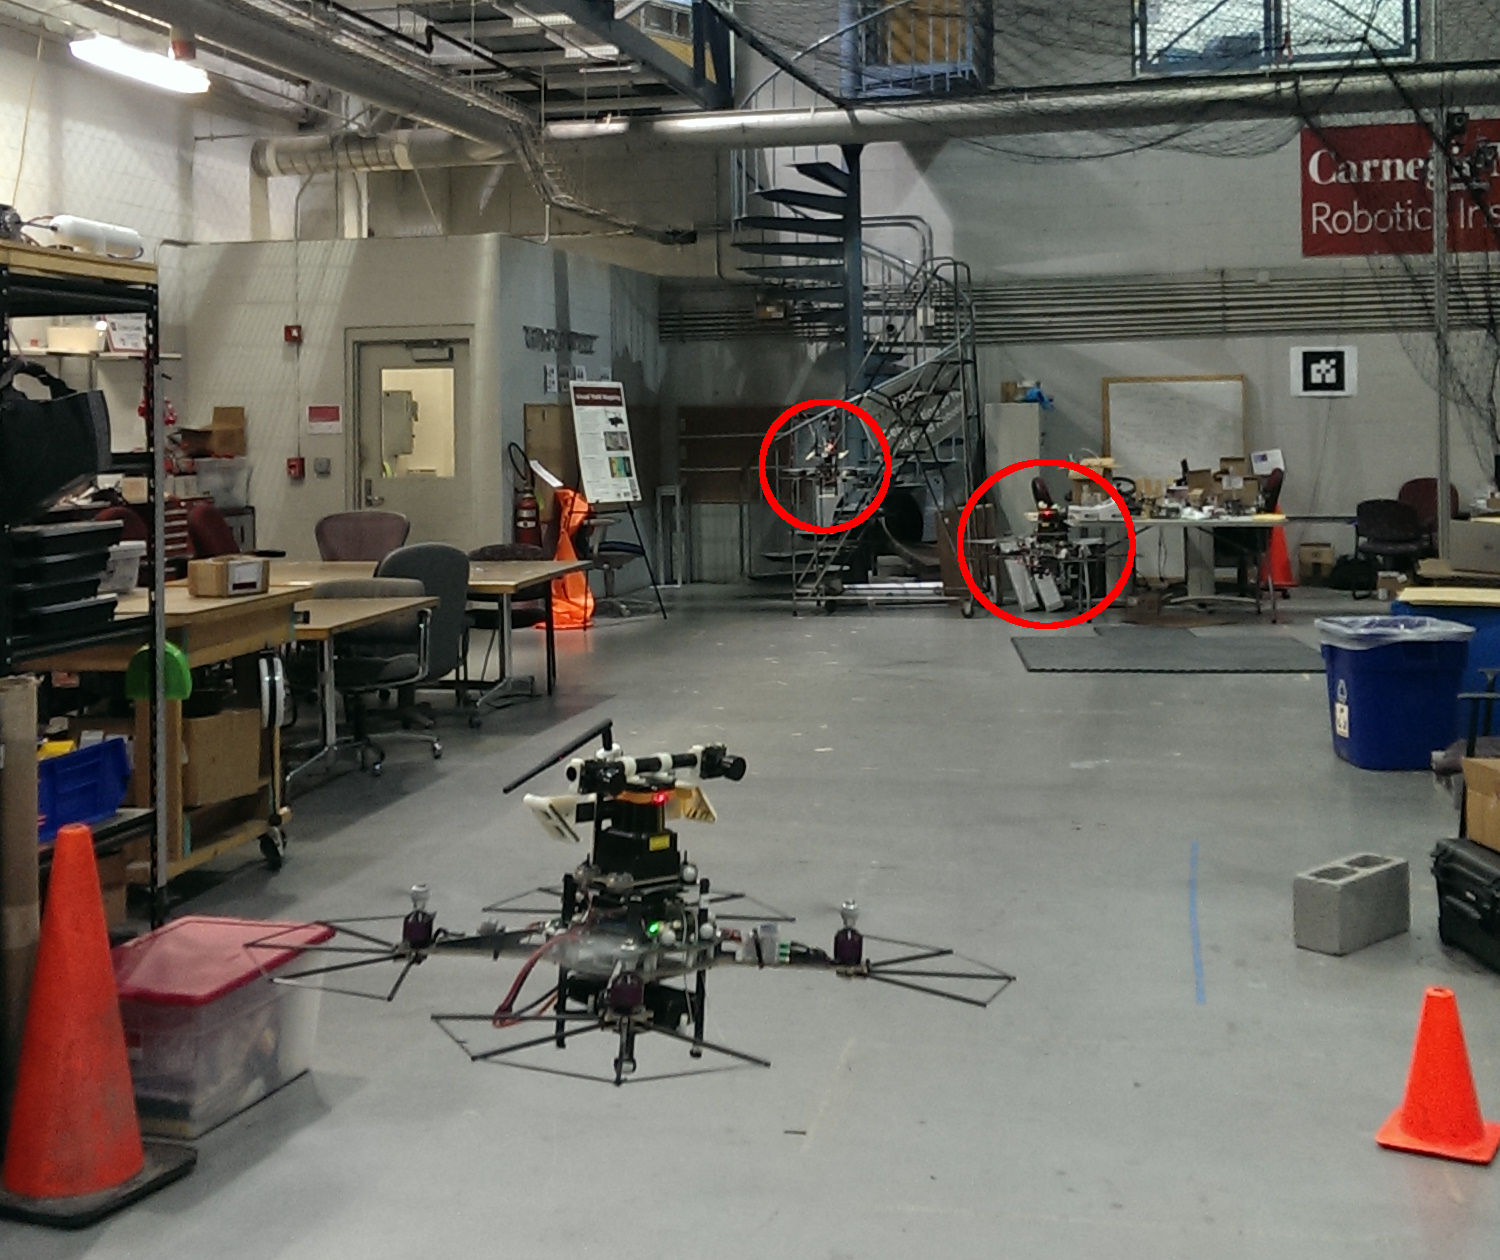
\includegraphics[width=2.5in]{3quads.png}
%\caption{Simulation Results}
%\label{fig_sim}
%\end{figure}
%\begin{table}[!t]
%\renewcommand{\arraystretch}{1.3}
%\caption{An Example of a Table}
%\label{table_example}
%\centering
%\begin{tabular}{|c||c|}
%\hline
%One & Two\\
%\hline
%Three & Four\\
%\hline
%\end{tabular}
%\end{table}

%\appendices
%\section{Proof of the First Zonklar Equation}

%\begin{thebibliography}{1}

%\bibitem{IEEEhowto:kopka}
%H.~Kopka and P.~W. Daly, \emph{A Guide to \LaTeX}, 3rd~ed.\hskip 1em plus
%  0.5em minus 0.4em\relax Harlow, England: Addison-Wesley, 1999.
%\end{thebibliography}